% ============================================================
% 片段：s03b  对应原文 section2.tex 第 878--1044 行；PDF 第 32--37 页
% 内容：§3.2 't Hooft 反常与 SPT 的一般分类（3.2.1--3.2.4）
% 译者：t-s03b   审校状态：初稿
% ============================================================

% ==== 原文 PDF 第 32 页（续；本片段自 §3.2 标题起）====
\subsection{'t Hooft 反常与 SPT 的一般分类}\label{sec:gen-SPT}

前面讨论的是具有 0-形式对称性 $G$ 的物理系统的 't Hooft 反常。't Hooft 反常由与规范联络的规范变换、或与群的 TDN 的局域移动相联系的相位因子刻画。我们也说明了，该相位因子对应于高一维 $G$-SPT 配分函数的构造数据。下面将把先前的讨论推广到更高维、高形式对称性、费米子系统与配边分类。这部分内容较为进阶，初学者不妨稍后再重读本节。

\subsubsection{更高维}

这一构造可以直接推广到 $d$ 维时空中的 't Hooft 反常。此时，先对 $d$ 维时空流形作三角剖分；再通过对该剖分的每一条边 $\langle ij \rangle$ 指定一个群元 $g_{ij}$，构造 $G$ 联络的 TDN。在局域重剖分（例如 Pachner 移动）下，这些联络应当彼此等价；但系统会相差一个 $U(1)$ 相位因子 $\omega_{d+1}$。该相位因子刻画系统中 $G$ 对称性的 't Hooft 反常。

此外，$d$ 维剖分的 Pachner 移动可以粘成一个 $(d+1)$ 维单纯形（simplex）。该 $(d+1)$ 维单纯形可理解为高一维 $G$-SPT 配分函数的构造单元。于是，$d$ 维 't Hooft 反常与高一维 $(d+1)$ 维 $G$-SPT 相之间出现直接联系。与 0+1 维中的结合律类似，相容方程由相位因子 $\omega_{d+1}$ 的上闭链条件 $\dd \omega_{d+1}=1$ 刻画。此外，还可对这些相位因子作规范变换，这等价于模去所有 $(d+1)$-上边缘。因此，$d$ 维 't Hooft 反常与 $d+1$ 维 $G$-SPT 相（在低维时）都由 $(d+1)$ 维群上同调分类~\cite{chen2012symmetry,chen2013symmetry}
\be\label{eq:HSPT}
H_{\mathrm{grp}}^{d+1}(G,U(1)) \cong H^{d+1}(BG,U(1)) \cong [BG,B^{d+1}U(1)].
\ee

% ==== 原文 PDF 第 33 页 ====
这里，$H_{\mathrm{grp}}^{d+1}$ 表示群上同调，$H^{d+1}$ 表示拓扑空间通常的（奇异）上同调，而 $[X,Y]$ 表示拓扑空间 $X$ 到 $Y$ 的连续映射的同伦类。

\begin{yizhu}式~\eqref{eq:HSPT} 的两个同构各有实质内容。左端 $H^{d+1}_{\mathrm{grp}}(G,U(1))\cong H^{d+1}(BG,U(1))$ 是群上同调与分类空间上同调之间的标准等同。右端之所以给出上同调，是因为 $B^{d+1}U(1)$ 就是 Eilenberg--MacLane 空间 $K(\mathbb{Z},d+2)$（由 $U(1)=K(\mathbb{Z},1)$ 逐次取分类空间，同伦群次数抬高 $d+1$），故 $[BG,B^{d+1}U(1)]\cong H^{d+2}(BG,\mathbb{Z})\cong H^{d+1}(BG,U(1))$，其中用到 $H^{k}(X,U(1))\cong H^{k+1}(X,\mathbb{Z})$。原文括注“in low dimensions”提示这是低维才成立的结论：维数升高后，群上同调只捕捉 SPT 分类的一部分，漏掉的部分（例如配边群中的自由部分）须由本小节最后讨论的配边分类补足。\end{yizhu}

\subsubsection{高形式对称性}

$d$ 维时空中的 $p$-形式对称性有直接的推广。此时，用阿贝尔群 $G$ 的元素标记三角剖分后时空的 $(p+1)$ 维单纯形。这一标记等价于指定一个映射 $A: M^d \rightarrow B^{p+1}G$，其中 $A$ 可视为 $(p+1)$-形式规范场。当系统作重剖分或 Pachner 移动（代表等价联络之间的规范变换）时，其变化由一个相位因子 $\omega_{d+1}$ 刻画。

与重剖分相联系的相位因子 $\omega_{d+1}$，可理解为构造 $p$-形式 $G$-SPT 配分函数时 $(d+1)$ 维单纯形的相位因子。相容条件给出 $\omega_{d+1}$ 的上闭链条件：$\mathrm{d} \omega_{d+1} = 1$。模去反项重定义（即上边缘）后，$p$-形式 't Hooft 反常与高一维的 $p$-形式 SPT 相都由下式分类：
\be
H^{d+1}(B^{p+1}G,U(1)) \cong [B^{p+1}G,B^{d+1} U(1)].
\ee
该式是式~(\ref{eq:HSPT}) 从 0-形式对称性到 $p$-形式对称性的直接推广~\cite{thorngren2015higher,kapustin2017higher}。

\subsubsection{费米子系统}

$d$ 维时空中 't Hooft 反常与 $(d+1)$ 维时空中 SPT 相之间的关系并不限于玻色子系统，它也延伸到费米子系统。

与玻色子系统相比，费米子系统的对称性结构更为复杂。与玻色子系统不同，费米子系统总具有一个由费米子宇称 $(-1)^F$ 生成、不可破缺的对称性 $\mathbb{Z}_2^f$。一般的费米子对称性 $G_f$ 是费米子宇称与玻色对称性 $G_b$ 的扩张，它可由短正合列（short exact sequence）分类~\cite{wang2020construction}：
\be
1\rightarrow \mathbb Z_2^f \rightarrow G_f \rightarrow G_b \rightarrow 1,
\ee
该扩张由 2-上闭链 $\lambda_2\in H^2_\mathrm{grp}(G_b,\mathbb Z_2^f)$ 支配。

\begin{yizhu}此处“分类”的准确含义是：固定 $G_b$ 后，$G_f$ 作为 $G_b$ 扩张的同构类由群上同调 $H^2_{\mathrm{grp}}(G_b,\mathbb{Z}_2^f)$ 分类，$\lambda_2$ 即该扩张的上闭链代表。物理上 $\mathbb{Z}_2^f$ 必为 $G_f$ 的中心子群（费米子宇称与任何对称性算符对易），故这是中心扩张；$\lambda_2$ 决定玻色对称性在费米子算符上的投影表示（即作用可相差一个费米子宇称相位），其杯积 $\lambda_2\smile n_d$ 并整体进入后文费米子 SPT 相容条件 (3.23) 右端的指数。核对原文时勿把 $\lambda_2$ 当作普通群元。\end{yizhu}

鉴于 't Hooft 反常与 SPT 相之间的关系，要理解费米子系统中的 't Hooft 反常，可以研究高一维的费米子 SPT 相。
% ==== 原文 PDF 第 34 页 ====
与用群上同调分类玻色子系统类似，费米子 SPT 相也存在一种分类，它利用一般群超上同调（general group super-cohomology）作为广义上同调理论~\cite{gu2014symmetry,wang2018towards,Xiong_2018,gaiotto2019symmetry,wang2020construction}。

在这一分类方案中，会用到多层上同调群。例如，玻色 SPT 相可以看作费米子 SPT 相，尽管它在费米子系统中可能变得平凡。因此，最高层对应于玻色层，由 $\omega_{d+1} \in H^{d+1}(G,U(1))$ 表示。此外还存在一个独特的超上同调层，由 $n_d \in H^d(G,\mathbb{Z}_2)$ 表示。这一层本质上涉及把复费米子装饰到时空中 TDN 的相互作用线上。$n_d$ 与 $\omega_{d+1}$ 之间的关系由相容条件约束。在 1+1 维反常或 2+1 维费米子 SPT 相的情形，该条件取一种特殊形式，称为超五边形方程（super-pentagon equation）~\cite{gu2014lattice,gu2015classification}。更一般地，费米子 SPT 相的相容条件表示为~\cite{gu2014symmetry,wang2020construction}
\be
\dd \omega_{d+1} = (-1)^{\lambda_2 \smile n_d + Sq^2(n_d)},
\ee
这里，$Sq^2(n_d) = n_d \smile_{d-2} n_d$ 表示 Steenrod 平方（Steenrod square）的上同调操作~\cite{steenrod1947products}，它与高阶杯积（higher cup product）有关。值得注意的是，该式表明 $\omega_{d+1}$ 不再是上闭链，而只是上链。

第三层通常称为马约拉纳层或 Kitaev 链层，记作 $n_{d-1} \in H^{d-1}_\mathrm{grp}(G_b,\mathbb{Z}_2)$，它起着关键作用。这一层涉及把 Kitaev 链装饰到时空中 TDN 的相互作用面上，从而给支配 $n_d$ 与 $\omega_{d+1}$ 的方程引入额外的扭曲。尽管这一层的障碍函数在低维已为人熟知~\cite{wang2018towards,wang2020construction,kapustin2017fermionic,brumfiel2016pontrjagin,brumfiel2018pontrjagin}，但随着维数升高，它们会变得明显更加复杂。

此外，除了必须满足相容方程，还须计入源于局域反项的上边缘的“规范变换”。值得注意的是，费米子系统呈现出更复杂的规范冗余网络。原则上，只要存在一个反常 SPT 态位于另一个 SPT 态的边界上，该边界 SPT 态就应视为平凡的~\cite{wang2019anomalous}。这是因为存在一个对称的、费米子的局域幺正变换，把该态连接到乘积态。

通过仔细计入这些障碍以及规范冗余（或平凡化），可以系统地构造并分类费米子 SPT 相，以及低一维系统中相应的 't Hooft 反常。

也可以把高形式对称性的研究推广到费米子系统，深入探讨高形式对称性保护的费米子拓扑相的分类。这一探讨与我们对低一维含费米子量子场论中高形式对称性 't Hooft 反常的理解密切相关。
% ==== 原文 PDF 第 35 页 ====
幸运的是，可以借用现有的数学工具，包括超上同调理论与自旋配边理论（spin cobordism），来处理这些费米子系统中的高形式对称性。推广的做法是把 $BG_b$ 换成 $B^{p+1}G_b$，以在所有装饰数据与障碍函数中容纳高形式规范场。重要的是，障碍函数本身保持不变，只是应理解为其自变量现在指由高形式规范场标记的相应单纯形。因此，所有构造与分类方案仍然适用。

\subsubsection{配边分类}

前面讨论了 $d$ 维 't Hooft 反常与 $(d+1)$ 维 SPT 相之间的对应，二者都由对称性的上同调群分类。然而，这一对应虽然在许多情形下是准确的，但在更高维会遇到局限。为处理这一点并提供更完备的框架，下面引入一个更精细的数学工具，即配边（bordism）。

考虑时空流形 $S^2$ 上一个 1+1 维 SPT 态。如前面所讨论，这类理论的配分函数由与剖分中每个三角形相联系的相位因子 $\omega_2$ 相乘得到。为说明这一点，可以先把二维球面 $S^2$ 剖分为单个四面体：
\begin{center}
    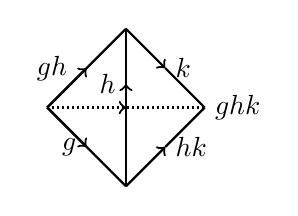
\begin{tikzpicture}
        \draw[->,thick] (0,0)--(0.5,-0.5) node[left]{$g$} ;
        \draw[thick] (0,0)--(1,-1)  ;
        \draw[->,thick] (1,-1)--(1,0.3) node[left]{$h$} ;
        \draw[thick] (1,0)--(1,1) ;
        \draw[->, thick] (1,1)--(1.5,0.5) node[right]{$k$};
        \draw[thick] (1.5,0.5)--(2,0) ;
        \draw[->, thick] (1,-1)--(1.5,-0.5) node[right]{$hk$} ;
        \draw[ thick] (1.5,-0.5)--(2,0);
        \draw[ thick,densely dotted] (0,0)--(2,0) node[right]{$ghk$};
        \draw[ thick,densely dotted,->] (0,0)--(1,0);
        \draw[ thick,->] (0,0)--(0.5,0.5) node[left]{$gh \ $};
        \draw[ thick] (0,0)--(1,1);
        % \node (a) at (5,0) {$ \mapsto  \ \ \omega_3(g,h,k)$.};
    \end{tikzpicture},
\end{center}
此时，配分函数 $Z[S^2]$ 由与该四面体相联系的各相位因子之积给出。数学上可写为：
\be Z[S^2] = \omega(g,h) \omega(gh,k)\omega^{-1} (g,hk) \omega^{-1} (h,k)=1. \ee
最后一步的关键观察是：$\omega_2$ 的上闭链条件得到满足，这保证配分函数等于 1。这意味着 $S^2$ 上的 1+1 维 SPT 态是平凡的。把这一过程递归地应用，可将结果推广到边界配分函数 $Z[\partial M_3]$，它同样等于 1。该结果不仅对 1+1 维成立，对更高维也成立。

\begin{yizhu}[原文疑误]正文称配分函数由每个三角形对应的相位因子 $\omega_2$ 相乘得到，但式 (3.24) 中出现的却是 $\omega$（未写下标 2），二者应指同一个 2-上闭链；译文照抄原文记号，建议核对原稿统一为 $\omega_2$。另外，式 (3.24) 的四个因子与四面体的四个面一一对应：以棱 $g,h,k,hk,gh,ghk$ 标记的四面体中，四个面按定向分别贡献 $\omega(g,h)$、$\omega(gh,k)$、$\omega^{-1}(g,hk)$、$\omega^{-1}(h,k)$，于是上闭链条件恰好使乘积为 1；初学者易漏掉两个 $\omega^{-1}$ 源于相应面的定向相反。\end{yizhu}

现在考虑边界分解 $\partial M_3 = M_2 \sqcup \overline{M_2'}$，可以利用两个取相反定向的面 $M_2$ 与 $\overline{M_2'}$ 把配分函数抵消掉。由此得到方程：
\be\ba  1 = Z[{M_2}]\cdot Z[\overline{M_2'}]  &= Z[M_2]\cdot Z[M_2']^{-1}   \\  
\Rightarrow Z[M_2]  &=  Z[M_2'] \ea\ee
这一观察提示我们引入一个新的等价类。

% ==== 原文 PDF 第 36 页 ====
\begin{definition}
两个 $d$ 维流形 $M_d$ 与 $M_d'$ 若存在一个 $(d+1)$ 维流形 $M_{d+1}$，使得其边界可分解为 $\partial M_{d+1} = M_d \sqcup \overline{M_d'}$，则称二者\textbf{配边等价}（bordism equivalent）。
\end{definition}

属于同一配边类的两个流形，在这一拓扑构造下具有相同的配分函数。此外，我们定义

\begin{definition}
流形的配边环（bordism ring）是三元组 $(\Omega_n^{SO},\sqcup,\times)$。$\Omega_n^{SO}$ 表示 $n$ 维定向流形模去配边等价关系所得的集合。运算 $\sqcup$ 表示不交并，在配边环中充当“加法”运算。运算 $\times$ 对应于笛卡尔积，在配边环中充当“乘法”运算。
\end{definition}

在构造可逆拓扑相（invertible topological phase）时，我们不仅考虑流形，还考虑配有平坦 $G$-联络的流形。此时，理论对每条边指定群 $G$ 中的一个值，并受平坦性条件约束。于是有映射：
\be  A: M_n/{\rm \{ bordism \ equivalence\} } \to BG.   \ee
类似地，可以定义配有平坦 $G$-联络的流形的配边类。相应的配边群记作 $\Omega_n^{SO}(BG)$，它要求联络在体 $M_{n+1}$ 与边界上都相容。

具有对称性 $G$ 的可逆拓扑相的配分函数 $Z$，定义为从配边群到 $U(1)$ 的映射：
\be\label{eq:cobor}  Z: \Omega_n^{SO}(BG)\rightarrow U(1).   \ee
该配分函数使我们能按上述映射的同构类对可逆拓扑序（invertible topological order）分类。该分类由配边群 $\Omega^n_{SO}(BG)$ 表示，它是配边群的 Pontryagin 对偶（Pontryagin dual）。若不计具体的规范群 $G$，并考虑 $BG$ 退化为一个点 $pt$ 的情形，则由于从任何空间到点的映射只有一个，有 $\Omega^n_{SO}(pt) = \Omega^n_{SO}$。

高一维的 't Hooft 反常与 SPT 相由配边描述~\cite{Kapustin:2014tfa,Kapustin:2014dxa,kapustin2014symmetry,freed2014shortrange,brumfiel2016pontrjagin,campbell2017homotopy,brumfiel2018pontrjagin,Wan:2018bns,Wan:2019soo,yonekura2019cobordism,freed2021reflection}。这一新的分类不仅计入 $G$-联络的变化，还允许时空流形本身的拓扑发生变化。它刻画了对称性 $G$ 与底层时空结构之间错综复杂的相互作用，为理解 't Hooft 反常与 SPT 相提供了完备的框架。

% ==== 原文 PDF 第 37 页 ====
另一方面，上同调分类是一种常常更易计算的近似。一般地，存在从群上同调分类到配边分类的群同态；但该群同态既不是单射也不是满射。好消息是，在低维，这个映射是同构，因此两种分类重合。

\begin{example}
一个点的配边群的最简单例子列举如下。
\begin{table}[htbp]
    \centering
    \begin{tabular}{|c|c|c|c|c|c|c|c|c|c|}
    \hline
        $n $ & $0$ & $1$ & $2$ & $3$ & $4$ & $5$ & $6$ & $7$ & $8$ \\
        \hline
        $\Omega_n^{SO}(pt)  $ & $\bbZ$ & $0$ & $0$ & $0$ & $\bbZ$ & $\bbZ_2$ & $0$ & $0$ & $\bbZ^2$ \\
        \hline
        % & $n_{\rm pts+}-n_{\rm pts-}$ &&&& $p_1$ & $w_2 w_3$ &&& $\bbC\bbP^4$, $\bbC\bbP^2\times \bbC\bbP^2$\\
        % \hline
    \end{tabular}
    \caption{一个点的配边分类列表。（原文 Table~1，PDF 第 37 页）}
    \label{tab:bordpts}
\end{table}

在这一例子中，零维由带 $\pm$ 方向的点的数目之差分类（一对 $+$ 方向与 $-$ 方向的点相互抵消）；4 维由第一 Pontryagin 类 $p_1$ 分类；5 维则由 Stiefel--Whitney 类的乘积 $w_2w_3$ 对流形分类。
\end{example}

一般地，$\Omega^n(BG)$ 的分类可能相当复杂。然而存在一种称为 Atiyah--Hirzebruch 谱序列（Atiyah-Hirzebruch spectral sequence）的实用方法，它使我们能利用前面已讨论的低维 $\Omega^n(pt)$ 的知识来计算 $\Omega^n(BG)$。Atiyah--Hirzebruch 谱序列有一个物理解释：把玻色可逆相装饰到群 $G$ 的畴壁上~\cite{chen2014symmetry, wang2021domain}。这一方法为理解并分类对称性及其相关拓扑序提供了有用的工具。

\begin{yizhu}表~\ref{tab:bordpts} 给出的是配边群 $\Omega_n^{SO}(pt)$ 本身（下标群），而 SPT 相的分类实际用的是它的 Pontryagin 对偶 $\Omega^n_{SO}(pt)=\mathrm{Hom}(\Omega_n^{SO}(pt),U(1))$（上标群）：自由部分 $\mathbb{Z}$ 对偶出 $U(1)$（连续的 $\theta$ 角型不变量），挠部分 $\mathbb{Z}_2$ 自对偶出 $\mathbb{Z}_2$（离散不变量），故表中 $n=4,8$ 的自由项与 $n=5$ 的 $\mathbb{Z}_2$ 项在物理上含义不同。表中非零项可由示性类读出：$\Omega_4^{SO}=\mathbb{Z}$ 由第一 Pontryagin 类 $p_1$ 探测，$\Omega_5^{SO}=\mathbb{Z}_2$ 由 $w_2w_3$ 探测，$\Omega_8^{SO}=\mathbb{Z}^2$，而 $n=1,2,3,6,7$ 均为零。要用 $\Omega^n(pt)$ 算出 $\Omega^n(BG)$，靠的是 Atiyah--Hirzebruch 谱序列：其 $E^2$ 页为 $E^2_{p,q}=H_p(BG,\Omega_q^{SO}(pt))$，收敛到 $\Omega_{p+q}^{SO}(BG)$；物理上即把 $q$ 维玻色可逆相装饰到 $G$ 的 $p$ 维畴壁上，各阶微分 $d_r$ 给出装饰的障碍。这也说明，从群上同调分类到配边分类的同态一般既非单射也非满射，仅在低维重合。\end{yizhu}

上述 't Hooft 反常与 SPT 相的配边分类，至少可以在概念上容易地推广到高形式对称性。关键的修改是把 1-形式规范场 $A$ 换成 $(p+1)$-形式规范场；相应地，配边群现在记作 $\Omega_n(B^{p+1}G)$。实践中仍可利用 Atiyah--Hirzebruch 谱序列作为计算这些配边群、理解所涉高形式对称性的有用工具。这一推广使我们能探索广泛的拓扑现象，并对具有高形式对称性的奇异物质相分类。

在费米子系统的语境下，配边等价的概念推广到带有自旋结构（spin structure）或其他切结构（tangential structure）的流形。有趣的是，在低维，配边分类与一般群超上同调分类彼此重合。这一对应使我们能利用 Atiyah--Hirzebruch 谱序列提供的畴壁装饰图像，为计算费米子系统中的 't Hooft 反常提供更便捷的方法。
